% !TeX root = ../main.tex
\cleardoublepage
\chapter{数据分析}\label{ch:analysis}

上一章的正式试验(\ref{sec:exp-main}节)中测得了\SIrange{1800}{2600}{\V}电压下的多组数据,并经初步处理得到$F$ -- $p$曲线以及关键点。本章将重点探讨这些数据所揭示出的晶圆脱附的物理过程,并据此判断出数据曲线中的晶圆脱附点,进而得到“脱附背吹压强 -- 电压”数据点。



\section{典型$F$ -- $p$曲线分析}\label{sec:analysis-example}


\subsection{简单型}\label{sec:analysis-example-naive} % 图样图森破,拿衣服

图~\ref{fig:data-fp-2000-4}、图~\ref{fig:data-fp-2000-8}~所示的曲线明显可分为两部分:左下方的部分中,$p$缓慢上升的同时,$F$变化不大;而右方的部分中,$F$随$p$上升而快速上升;两部分中间有明显的转折点。除此转折点以外,可能还有其他的转折点,但对曲线整体走势影响不大。简单型曲线完全符合第\ref{ch:principle}章中对脱附判定的预测,然而实际情况表明,纯粹的简单型曲线占所有检测数据的比例非常小:虽然大部分数据走势与简单型类似,但其组成往往更复杂,在第一次出现$F$随$p$上升而快速上升(走势为向右上方)前后可能存在多个其他类型的转折点;这些特征将在其他曲线类型中介绍,并在\ref{sec:analysis-feature}节中加以分析。

\begin{figure}[tbh]
\centering
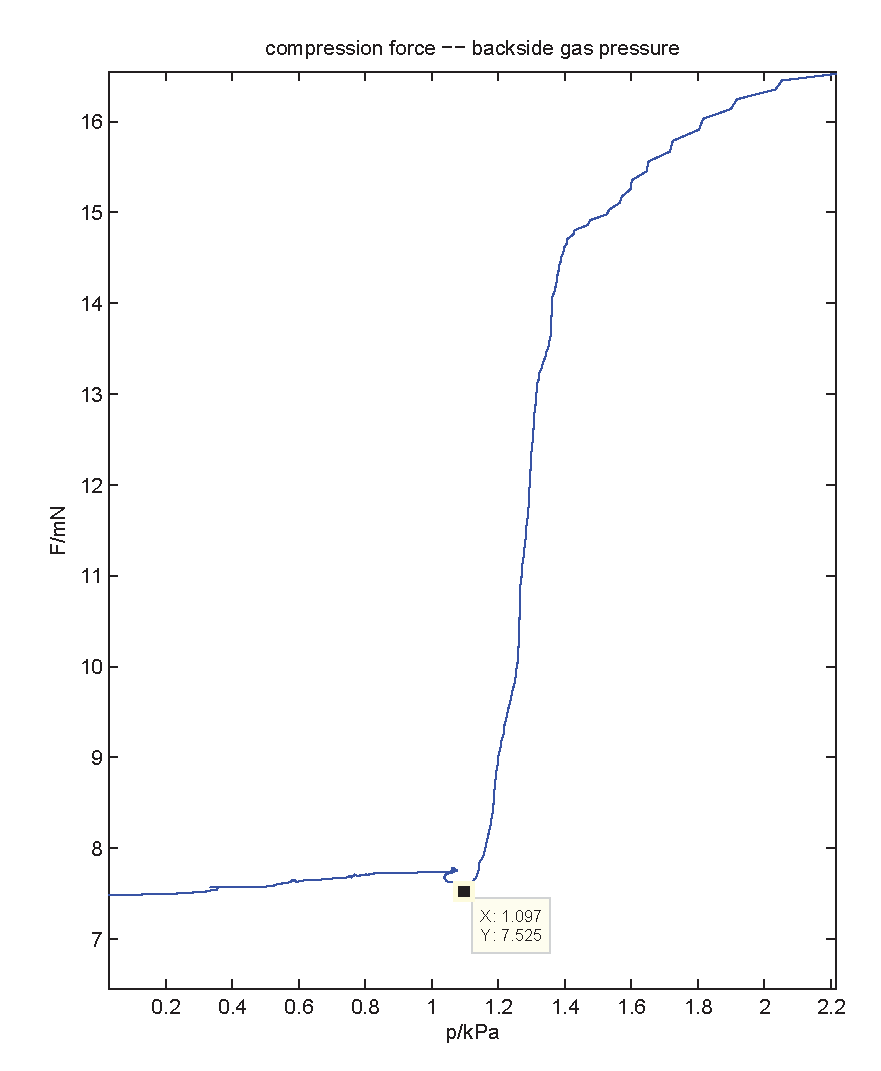
\includegraphics
  [max size={0.9\linewidth}{0.9\textheight}]
  {data/fp__2000__4}
\caption{探头受力随背吹压强变化曲线(\SI{2000}{\V} 第4组)}
\label{fig:data-fp-2000-4}
\end{figure}

\begin{figure}[p]
\centering
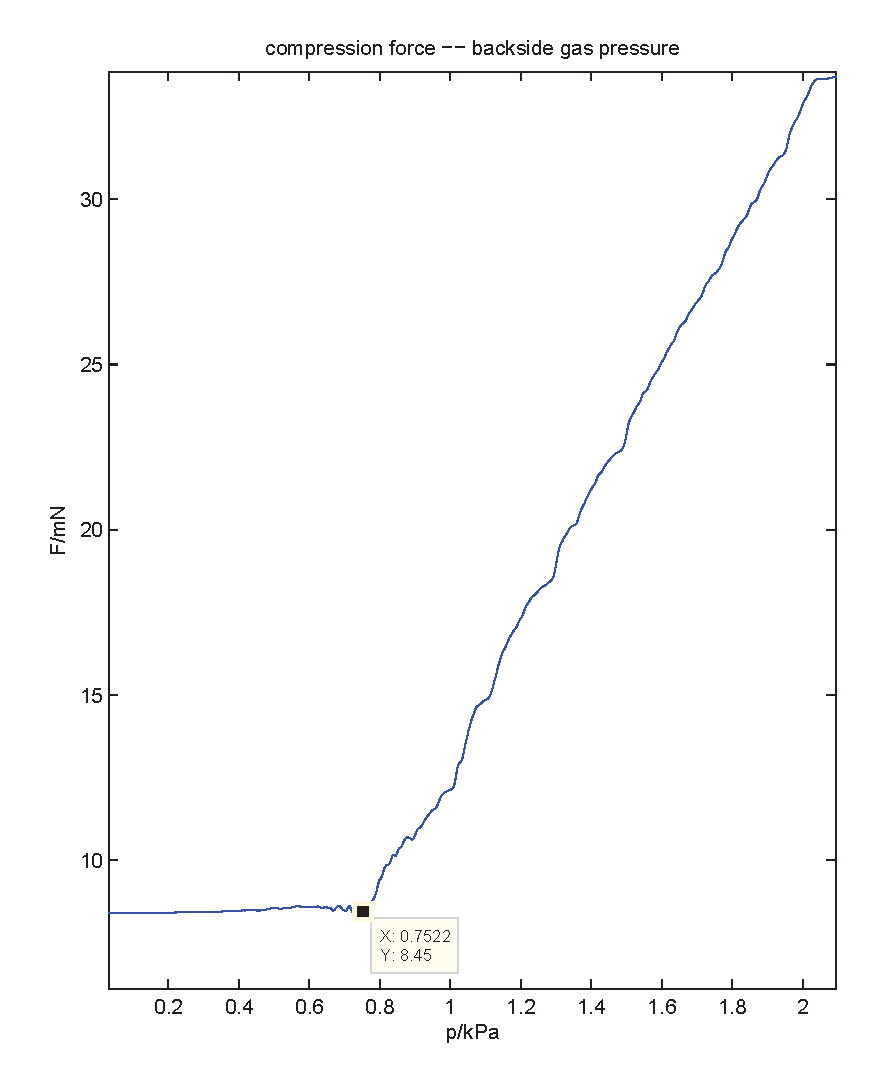
\includegraphics
  [max size={0.9\linewidth}{0.9\textheight}]
  {data/fp__2000__8}
\caption{探头受力随背吹压强变化曲线(\SI{2000}{\V} 第8组)}
\label{fig:data-fp-2000-8}
\end{figure}


\clearpage


\subsection{回转型}\label{sec:analysis-example-loop}

图~\ref{fig:data-fp-2400-2}、图~\ref{fig:data-fp-2600-2}~所示曲线中能明显观察到一个大回环,其走向为逆时针方向,即:随着试验继续,$p$由逐渐升高转为降低\footnotemark{}的同时,$F$出现一个尖峰,又迅速回落。该特征在很多组数据曲线中均为最明显的特征之一,尤其是在电压较高($V \geq \SI{2200}{\V}$)时。

\footnotetext{此时减压阀开度仍在增加,具体原因在后文中分析。}

\begin{figure}[tbh]
\centering
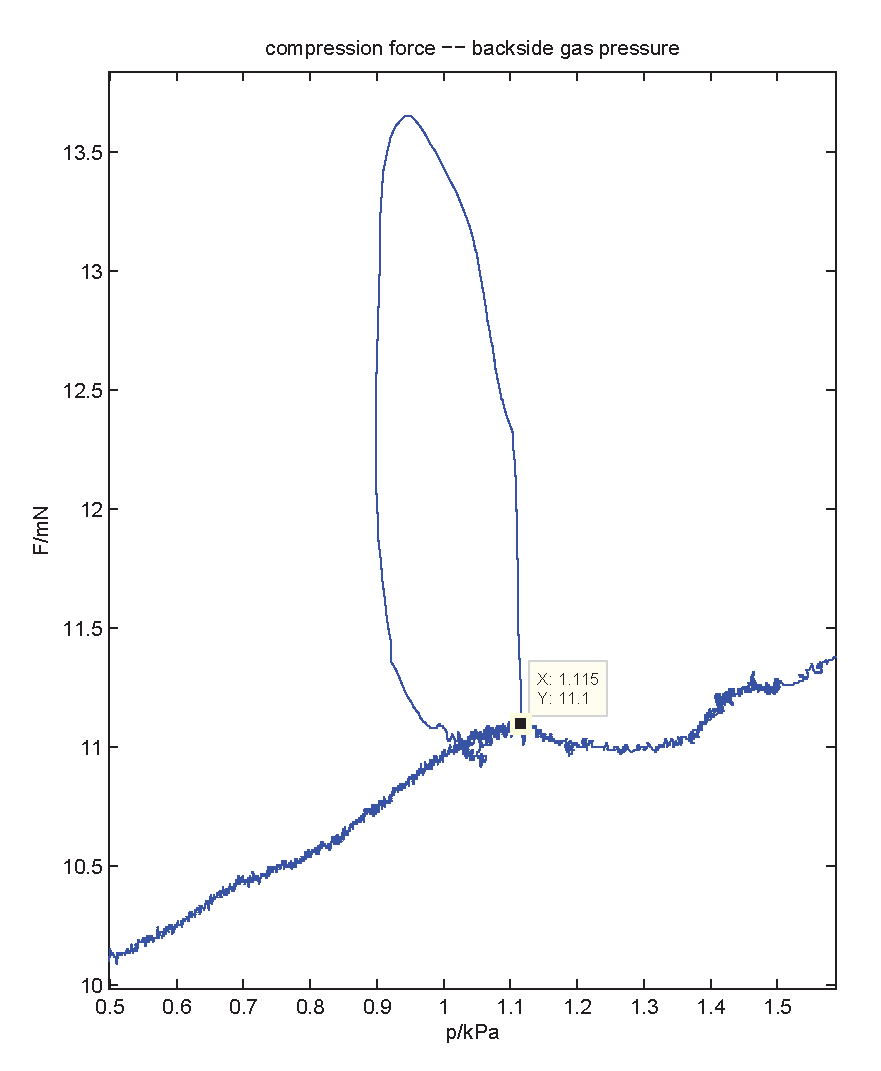
\includegraphics
  [max size={0.9\linewidth}{0.9\textheight}]
  {data/fp__2400__2}
\caption{探头受力随背吹压强变化曲线(\SI{2400}{\V} 第2组)}
\label{fig:data-fp-2400-2}
\end{figure}

\begin{figure}[p]
\centering
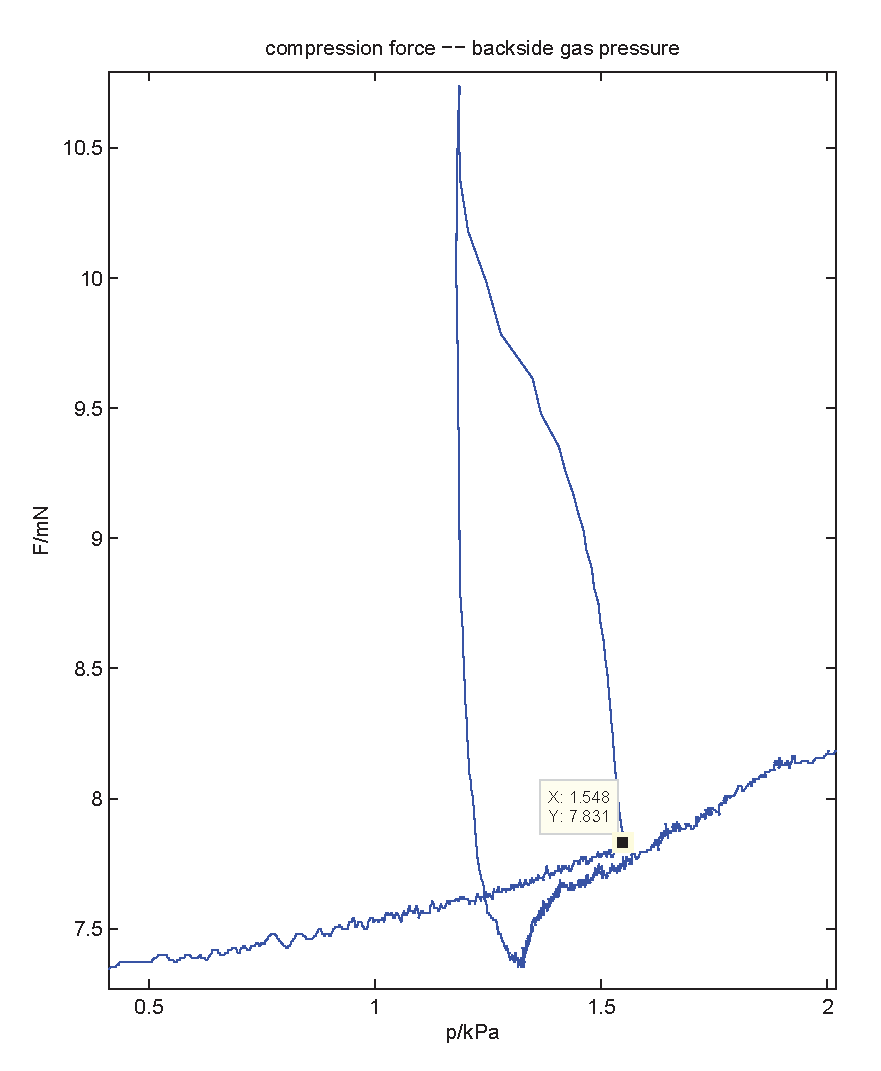
\includegraphics
  [max size={0.9\linewidth}{0.9\textheight}]
  {data/fp__2600__2}
\caption{探头受力随背吹压强变化曲线(\SI{2600}{\V} 第2组)}
\label{fig:data-fp-2600-2}
\end{figure}


\clearpage


\subsection{密集折点型}\label{sec:analysis-example-multi}

观察图~\ref{fig:data-fp-1800-10}、图~\ref{fig:data-fp-2000-7}~所示曲线,发现虽然整体走势与\ref{sec:analysis-example-naive}节中简单型相似,但在两部分曲线中间出现多个相距不远的折点。其他数据曲线中,虽然较少出现与简单型相似的走势,仍有很多具有密集折点特征。

\begin{figure}[tbh]
\centering
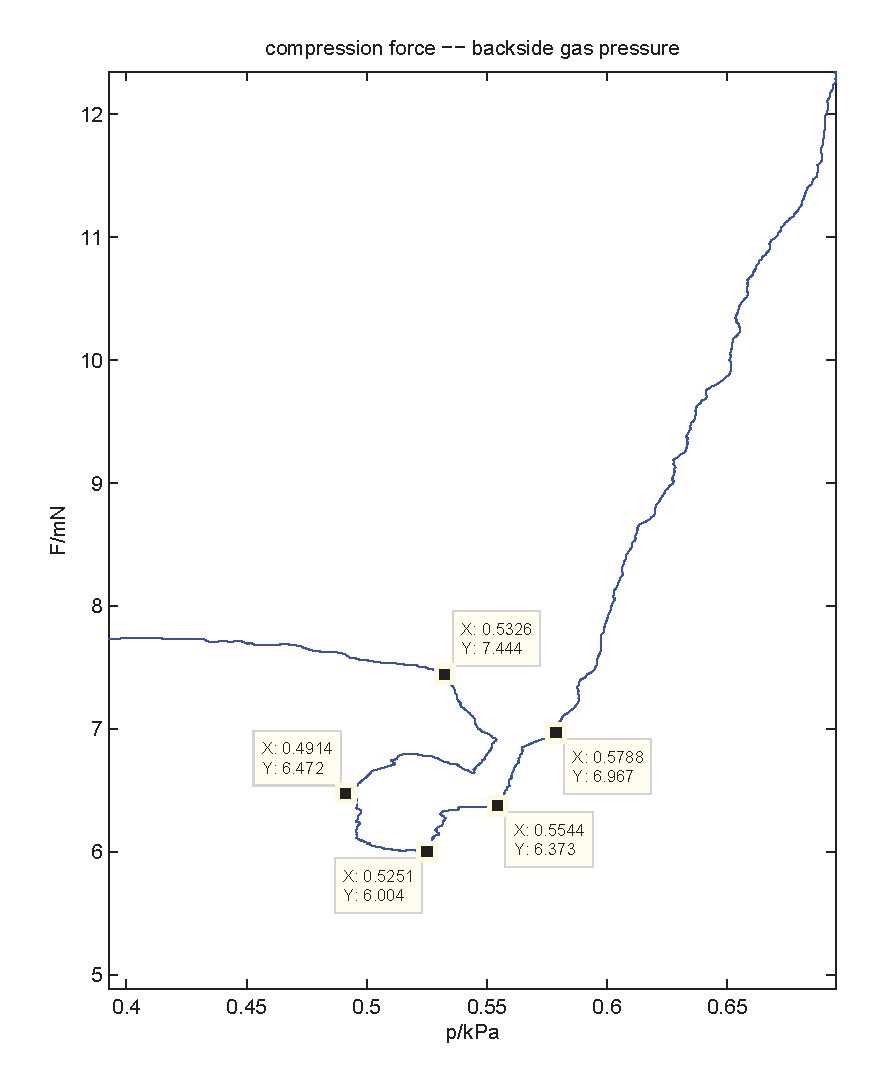
\includegraphics
  [max size={0.9\linewidth}{0.9\textheight}]
  {data/fp__1800__10}
\caption{探头受力随背吹压强变化曲线(\SI{1800}{\V} 第10组)}
\label{fig:data-fp-1800-10}
\end{figure}

\begin{figure}[p]
\centering
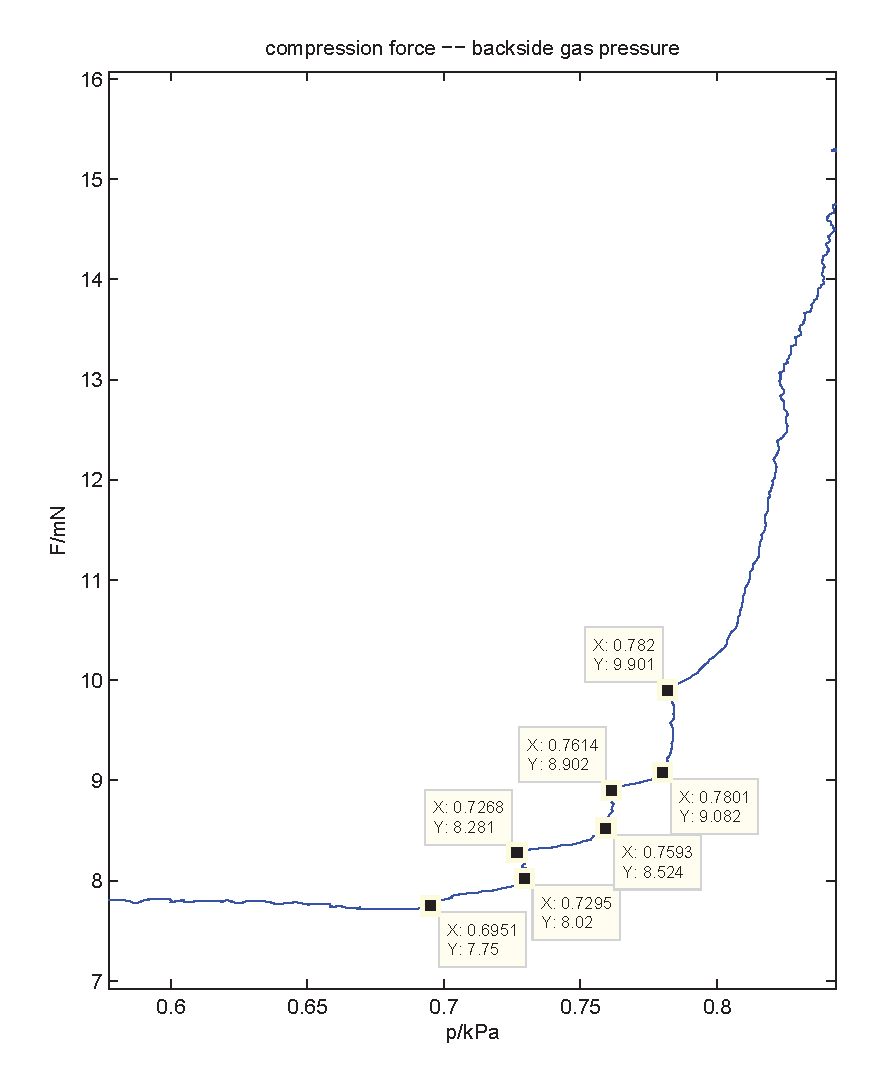
\includegraphics
  [max size={0.9\linewidth}{0.9\textheight}]
  {data/fp__2000__7}
\caption{探头受力随背吹压强变化曲线(\SI{2000}{\V} 第7组)}
\label{fig:data-fp-2000-7}
\end{figure}


\clearpage


\subsection{倒勾型}\label{sec:analysis-example-sawtooth}

图~\ref{fig:data-fp-2400-6}、图~\ref{fig:data-fp-2600-5}~所示的曲线走势与大部分数据曲线不同:在检测刚开始的时候,$F$即随$p$上升而上升,然后在一点突然出现转折,曲线总体趋势变为$p$上升而$F$反而快速下降。值得注意的是,该类曲线均满足$V \geq \SI{2200}{\V}$。

\begin{figure}[tbh]
\centering
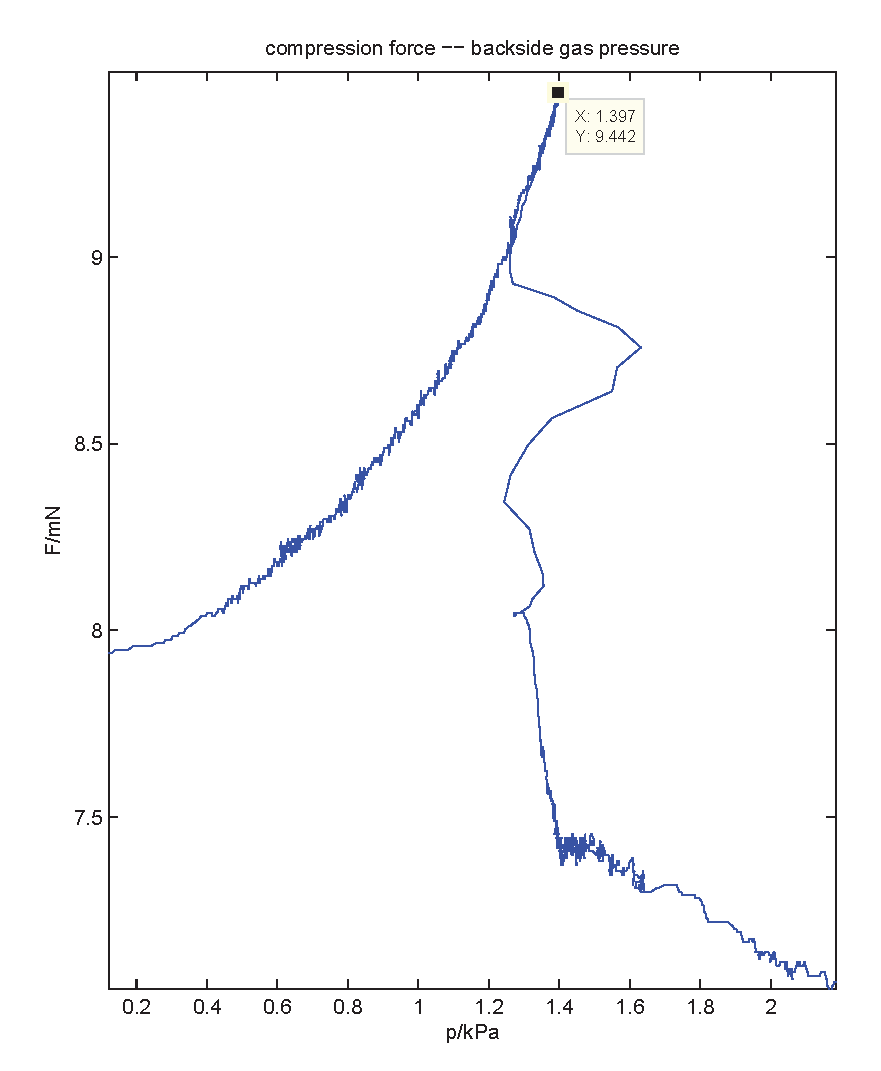
\includegraphics
  [max size={0.9\linewidth}{0.9\textheight}]
  {data/fp__2400__6}
\caption{探头受力随背吹压强变化曲线(\SI{2400}{\V} 第6组)}
\label{fig:data-fp-2400-6}
\end{figure}

\begin{figure}[p]
\centering
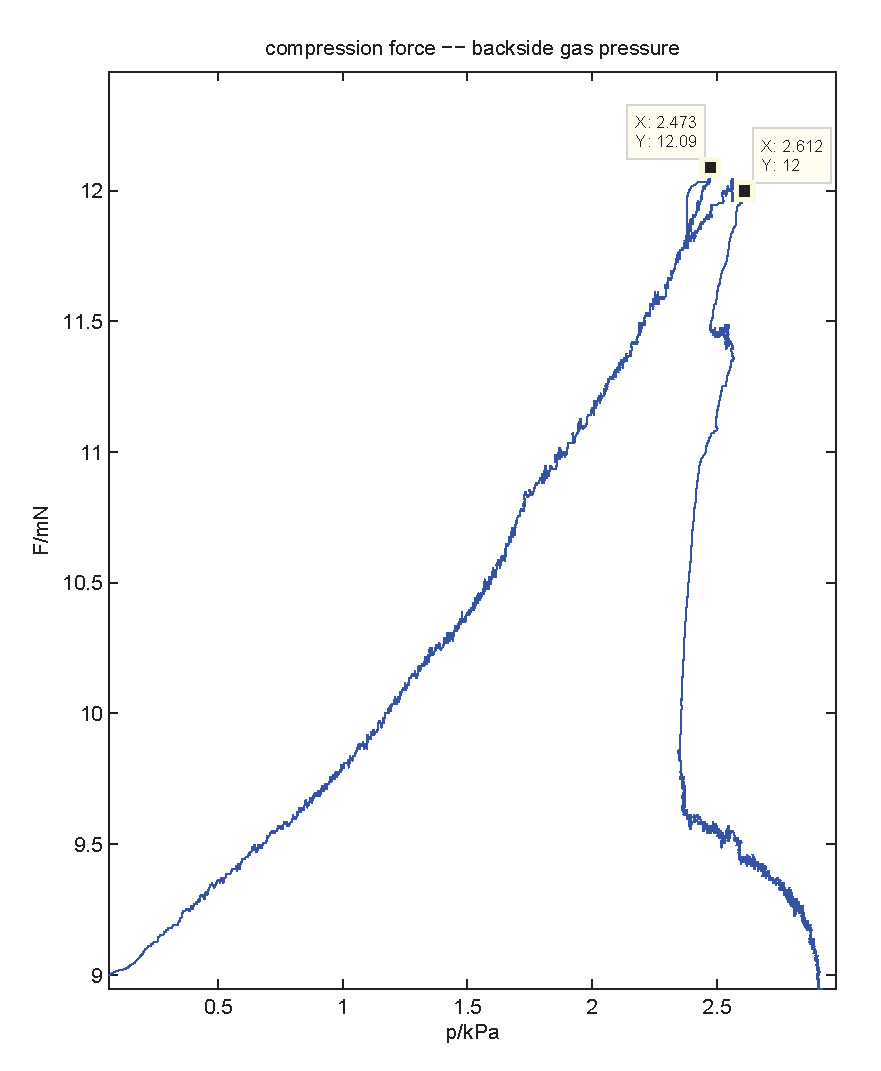
\includegraphics
  [max size={0.9\linewidth}{0.9\textheight}]
  {data/fp__2600__5}
\caption{探头受力随背吹压强变化曲线(\SI{2600}{\V} 第5组)}
\label{fig:data-fp-2600-5}
\end{figure}


\clearpage


\subsection{复合型}\label{sec:analysis-example-complex}

正式试验获得的数据中,少数$F$ -- $p$曲线走势较为复杂,包含多种特征,如:图~\ref{fig:data-fp-2200-6}、图~\ref{fig:data-fp-2200-7}~均可视为倒钩型、回转型、简单型的顺序组合;图~\ref{fig:data-fp-2400-7}可视为倒钩型、密集折点型与简单型的顺序组合等等。这类数据揭示了背吹平衡脱附过程本身的复杂性。
%,需通过对其组成特征的分析来加深对其内在物理过程的理解。

\begin{figure}[tbh]
\centering
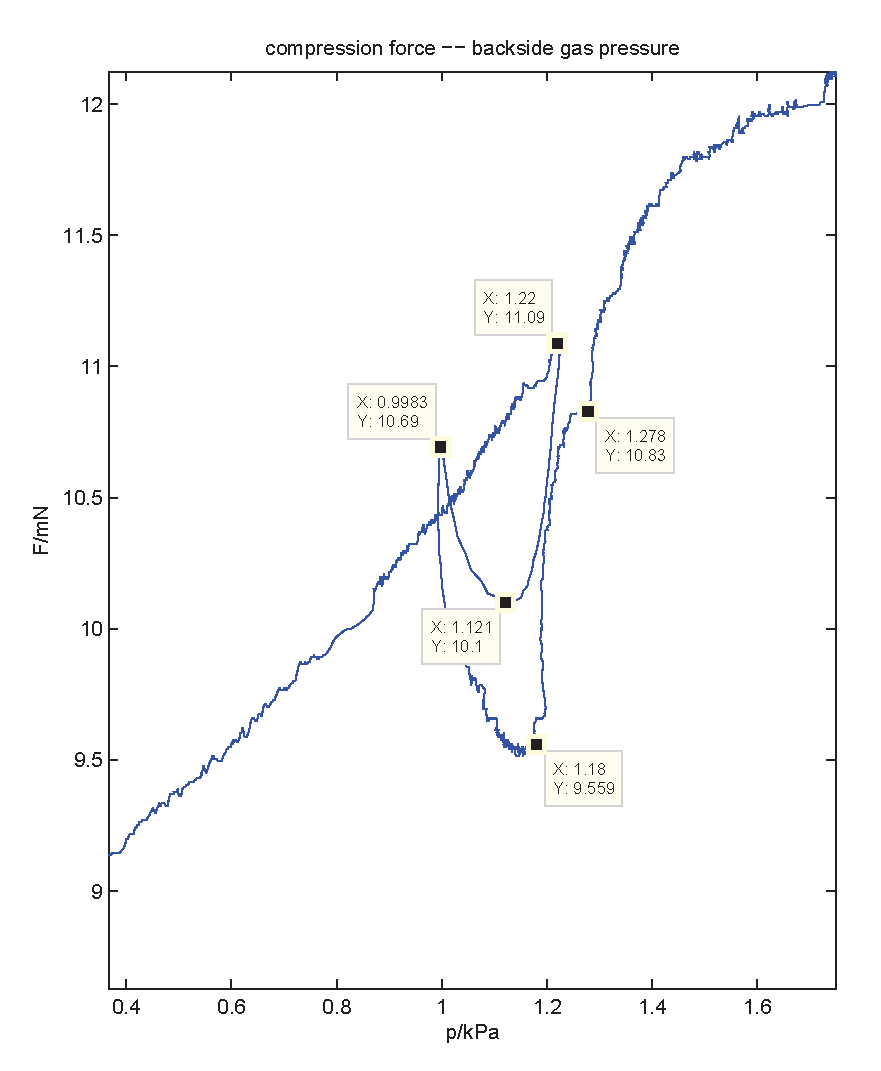
\includegraphics
  [max size={0.9\linewidth}{0.9\textheight}]
  {data/fp__2200__6}
\caption{探头受力随背吹压强变化曲线(\SI{2200}{\V} 第6组)}
\label{fig:data-fp-2200-6}
\end{figure}

\begin{figure}[tbh]
\centering
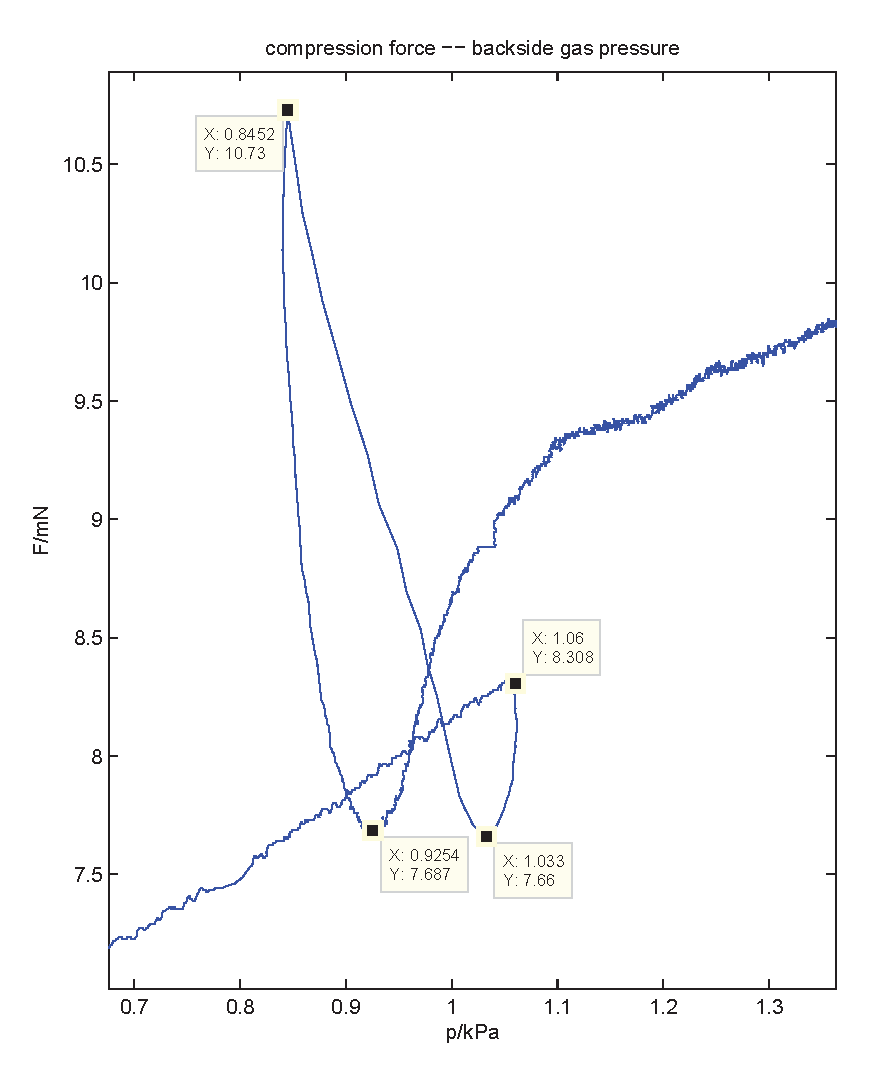
\includegraphics
  [max size={0.9\linewidth}{0.9\textheight}]
  {data/fp__2200__7}
\caption{探头受力随背吹压强变化曲线(\SI{2200}{\V} 第7组)}
\label{fig:data-fp-2200-7}
\end{figure}

\begin{figure}[p]
\centering
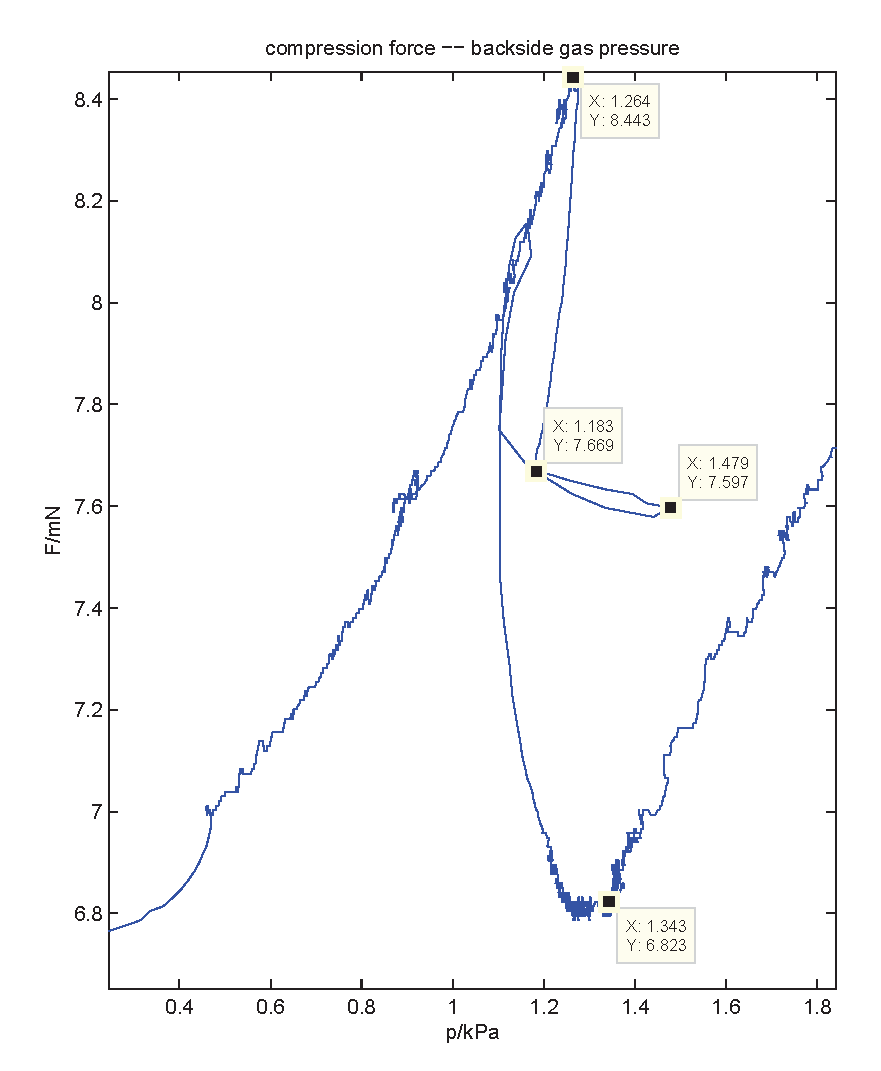
\includegraphics
  [max size={0.9\linewidth}{0.9\textheight}]
  {data/fp__2400__7}
\caption{探头受力随背吹压强变化曲线(\SI{2400}{\V} 第7组)}
\label{fig:data-fp-2400-7}
\end{figure}



\clearpage



\section{曲线特征与对应物理过程}\label{sec:analysis-feature}

本节将列举一些$F$ -- $p$曲线中较多出现的特征,并结合静电卡盘与检测平台的结构特点,提出关于其对应物理过程的合理猜想。


\subsection{简单失稳脱附}\label{sec:analysis-feature-destabilize}

当类似\ref{sec:analysis-example-naive}节中图~\ref{fig:data-fp-2000-4}~所示的$p$较小增长引起$F$较大增长的曲线段出现时,一种可能的解释是微力探头与晶圆接触处局部已发生较大尺度的脱附,且静电力与背吹压力构成的平衡不再稳定:随着静电力减小,间隙随之逐渐扩大,引起静电力进一步减小,仅由于晶圆本身刚度以及其他区域吸附力的影响,尚未完全脱附,此时再增加压强,则未能与静电力相平衡的压力将由微力探头对晶圆施加的接触力来平衡,导致$F$迅速随$p$增长。


\subsection{局部脱附 -- 再吸附}\label{sec:analysis-feature-reattach}

图~\ref{fig:data-fp-2000-10-crop}、图~\ref{fig:data-fp-1800-10-crop}~所示的特征在大多数曲线中均有出现,甚至出现多次,且一般为曲线中最早出现的特征。该特征曲线段特点为:折点之前$p$升高而$F$基本不变;当$p$达到一定值时,$F$开始降低,之后$p$也随之降低,直至$F$达到一个新的稳定值;此后$p$回升时,$F$保持新稳定值基本不变。该特征一般在图线中呈现为尺度较小但明显的“乙”或“已”字型。由于试验过程中保证减压阀开度始终单调增加,压强出现下降的原因只能是背吹通道流量增加,说明晶圆与静电卡盘边缘的间隙有所增加;同时,由于微力探头放置在晶圆与卡盘的中心,其受力下降说明晶圆中心处局部与静电卡盘的间隙有所下降。由此推测可能出现的现象是:随着压强增加,晶圆外围出现局部脱附现象(局部失稳),然而并未破坏整体平衡稳定性,之后晶圆在静电力作用下,改变了翘曲模式,进入了能量更低的继续维持稳定吸附的状态。

\begin{figure}[thbp]
\centering
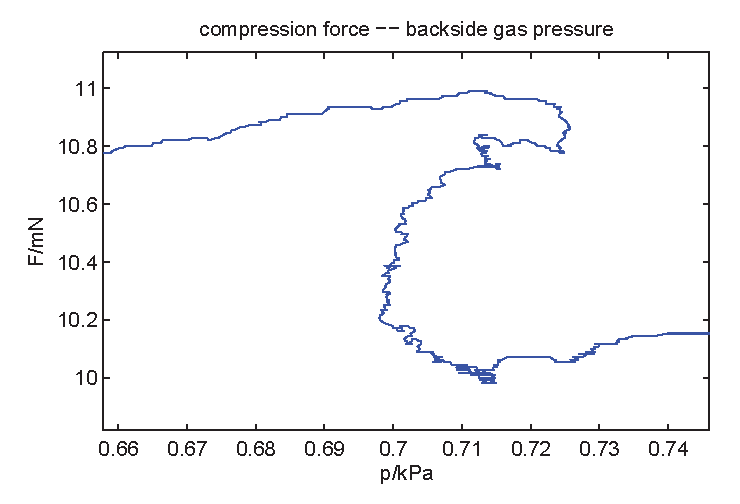
\includegraphics[width=0.8\linewidth]{data/fp__2000__10__crop}
\caption{探头受力随背吹压强变化曲线(\SI{2000}{\V} 第10组\ 局部放大)}
\label{fig:data-fp-2000-10-crop}
\end{figure}

\begin{figure}[thbp]
\centering
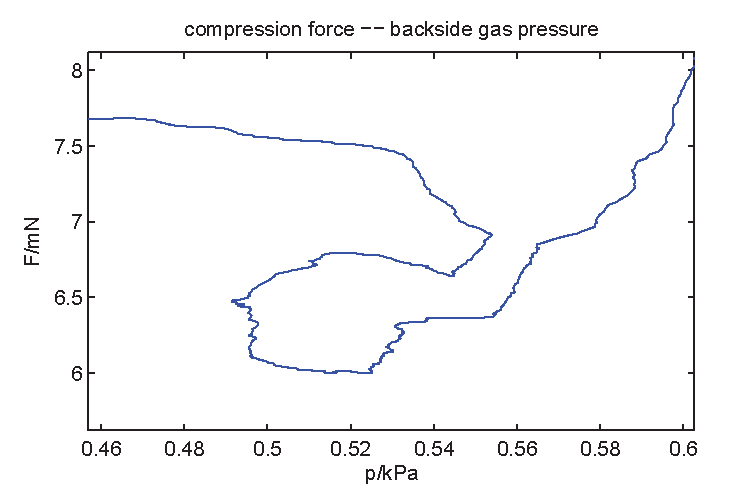
\includegraphics[width=0.8\linewidth]{data/fp__1800__10__crop}
\caption{探头受力随背吹压强变化曲线(\SI{1800}{\V} 第10组\ 局部放大)}
\label{fig:data-fp-1800-10-crop}
\end{figure}


\subsection{局部脱附 -- 整体脱附 -- 再吸附}\label{sec:analysis-feature-loop}

以下分析\ref{sec:analysis-example-loop}节所述的“回转”特征:折点之前$p$升高而$F$ 缓慢随之升高;当$p$达到一定值时,$F$突然急剧升高,同时$p$出现明显下降;之后$F$回落,$p$也在下降停止后略微回升,直到$F$达到一个新的稳定值,趋势恢复到与出现折点之前大致相同。采用与\ref{sec:analysis-feature-reattach}节中“乙”字特征相似的分析思路:最初阶段$F$有较为明显的上升,说明晶圆中心处局部间隙在逐步扩大,直至中心失稳脱附,$F$因此急剧升高;但同时在中心的带动下,边缘处间隙也随即扩大,出现整体脱附现象,导致背吹通道流量突增,压强降低,直至不足以与吸附力相平衡,晶圆重新回到稳定吸附状态。

“回转”特征与“乙”字特征的相同之处在于:均出现脱附与再吸附的现象,且再吸附后有可能比脱附前更稳定(静电力更大);不同之处在于:“乙”字特征仅出现局部脱附,而“回转”特征中出现了明显的整体脱附。


\subsection{快速断续脱附}\label{sec:analysis-feature-multi}

\ref{sec:analysis-example-multi}节中描述的“密集折点型”曲线中,有一类包含如图~\ref{fig:data-fp-2000-7}~所示的特征:在较小的压强范围内,交替出现$p$变化不大而$F$向上跳变、$p$上升而$F$基本不变或缓慢上升的两种曲线段,直至$F$跳变越来越大,出现失稳脱附(\ref{sec:analysis-feature-destabilize}节)。与失稳脱附的分析类比,该特征很可能对应晶圆中心局部间隙间断性扩大,逐步失稳并出现整体脱附的物理过程。


\subsection{边缘脱附}\label{sec:analysis-feature-rim}

一类较为复杂的曲线特征为\ref{sec:analysis-example-sawtooth}节中的“倒钩型”:$F$从加压开始就随$p$较快上升,但推测晶圆整体仍处于吸附状态;折点后,$F$迅速降低而$p$出现一定波动,说明晶圆中心区域间隙变小,吸附变强;突变过后,随$p$增加,$F$的趋势反而变为缓慢降低,因此推测在折点处,晶圆由“中心间隙较大,边缘间隙较小、整体保持吸附”的状态快速转变为“中心间隙较小且更牢固吸附,边缘脱附”的状态。此时,由于静电卡盘的氦气背吹孔布置在较外侧处(如图~\ref{fig:rig-model-echuck-helium}),而晶圆边缘已脱附,无法形成接触密封,导致流动大大增强,不能简单认为晶圆仅受静压强作用。此后过程的分析需要通过对晶圆表面各处挠度的测量,建立准确的CFD模型,并通过背吹系统的流量、压强信息,获得晶圆表面的受力分布,由于已超出本文范围,不再赘述。

\begin{figure}[thb]
\centering
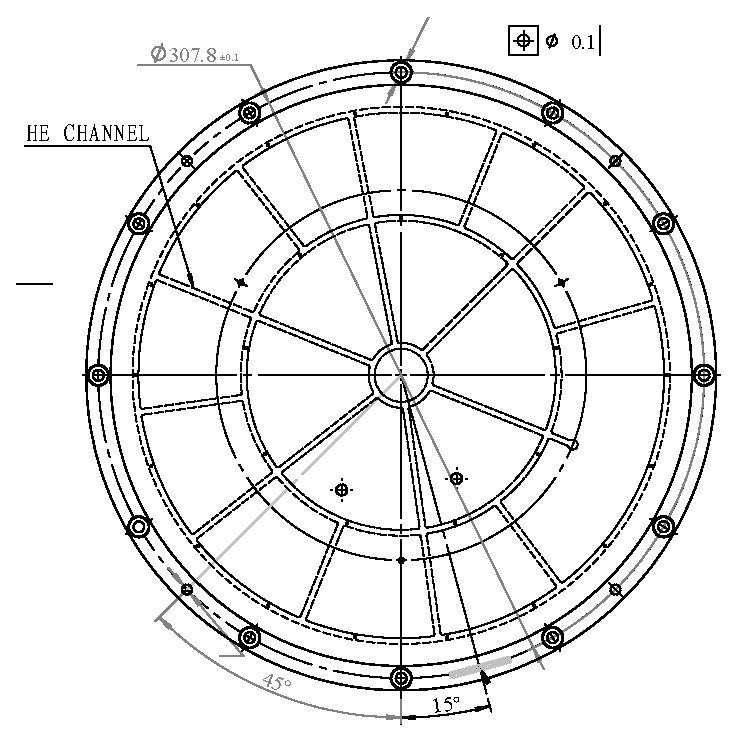
\includegraphics
  [max size={0.8\linewidth}{0.45\textheight}]
  {rig/model__echuck__helium}
\caption{静电卡盘背吹通道工程图}
\label{fig:rig-model-echuck-helium}
\end{figure}



\section{脱附点的判定}\label{sec:analysis-criterion}

由上一节中各特征的物理过程分析,可得出一般$F$ -- $p$曲线的脱附点判断方式:曲线中最早出现的“简单失稳脱附”特征(\ref{sec:analysis-feature-destabilize}节)、“回转”特征(\ref{sec:analysis-feature-loop}节)以及“边缘脱附”特征(\ref{sec:analysis-feature-rim}节)均标志着晶圆大面积失稳性脱附,因此取其关键折点作为脱附点:对于“简单失稳”特征,取其唯一的折点;对于“回转”特征,取其从平稳段转入回转段的折点;对于“边缘脱附”特征,可取$F$由升转突降的折点。若在“简单失稳脱附”特征前首先出现了“快速断续脱附”特征(\ref{sec:analysis-feature-multi}节),原则上说可舍弃该组数据\footnotemark{},但此处仍规定不舍弃数据时的脱附点选取为第一次出现$F$小范围跳变的折点。而对于“局部脱附 -- 再吸附”特征(\ref{sec:analysis-feature-reattach}节),由于对应物理过程中并未出现失稳脱附,反而使晶圆吸附更稳定,不将其作为脱附点判据。对于\ref{sec:analysis-example-complex}节所述的复合型曲线,可先检查曲线是否具有“简单失稳脱附”或“回转”特征,若有,则可直接判定其折点为脱附点;若没有,但存在“边缘脱附”特征,则取其折点为脱附点;若这些特征均未出现,暂时可判定该数据曲线无效,之后单独分析。

\footnotetext{断续脱附特征在试验中出现较少,目前猜想该现象是由颗粒污染引起,若能改善试验条件,有可能消除该特征的出现。}



\section{数据汇总与拟合}\label{sec:analysis-tally}

按照上文总结出的数据处理与分析方法,找出正式试验中所有有效数据的脱附点与对应的脱附压强,并绘制脱附压强 -- 电极电压 箱线图(图~\ref{fig:data-tally-box})。可见,同电压下多次检测得到的脱附压强较为分散,因此采用中位数估计同电压下的脱附压强真实值,并用二次多项式拟合,结果如图~\ref{fig:data-tally-fit},多项式为:
\[
\hat{p} = 0.05919\;\hat{v}^2 + -1.324\;\hat{v} + 1.000
\]
其中,$\hat{p} = p / \SI{1}{\kPa}$,$\hat{v} = v / \SI{1}{\kV}$;拟合相关系数$R^2 = \num{0.9992}$。相关系数较高,说明数据较好地符合拟合多项式,验证了检测方案与上述数据处理与分析方法的可行性。同时,考虑到在库仑型静电卡盘的静电力理论公式%
(见第\ref{ch:bg}章 \eqref{eq:bg-coulomb}式)%
中,静电力与电压平方成正比,即使排除掉重力、大气压强等常数项,仍无法解释拟合多项式中的一次项,说明实际静电力产生机理比理论公式复杂,仍有理论公式未能考虑到的因素,有待进一步研究以确定产生该偏差的原因。

\begin{figure}[thbp]
\centering
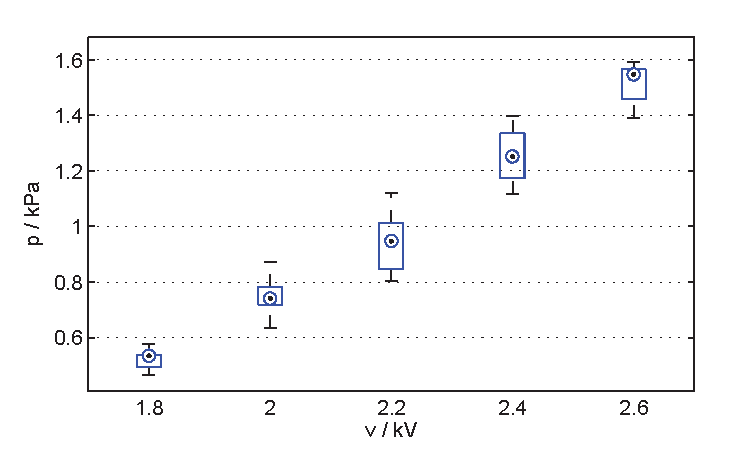
\includegraphics[width=0.8\linewidth]{data/tally__box}
\caption{脱附压强 -- 电极电压数据箱线图}
\label{fig:data-tally-box}
\end{figure}

\begin{figure}[thbp]
\centering
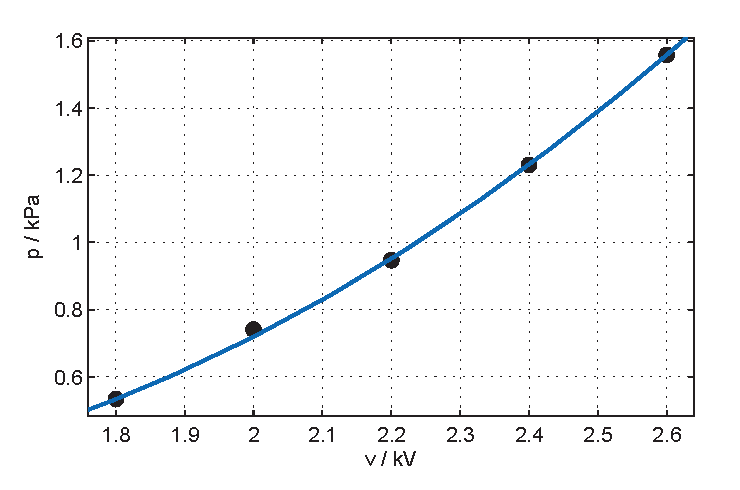
\includegraphics[width=0.8\linewidth]{data/tally__fit}
\caption{脱附压强 -- 电极电压数据拟合}
\label{fig:data-tally-fit}
\end{figure}



\section{本章小结}\label{sec:analysis-summary}

本章通过对正式试验中各$F$ -- $p$曲线的分析,将所有曲线按照其走势特点分为了5大类,并一一分析了能代表该类特征的典型曲线。然后,从中找出了这些曲线中出现的共有的5个特征,给出了对与其对应的晶圆可能的吸附与脱附物理过程的合理猜想,并通过对特征对应物理过程的分析,提出了判定$F$ -- $p$曲线的脱附点的一般方法。最后,将该方法应用于正式试验中获得的有效数据的处理中,得到了脱附压强 -- 电极电压的关系,并通过拟合处理,最终验证了检测方案设计、检测平台实现、以及数据处理与分析方法的可行性。